\begin{displayquote}
	\textsf{An important application on supercomputers is to solve the linear systems and eigenvalue problems. The chapter gives an overview of the relevant iterative methods to solve large-scale non-Hermitian linear systems and eigenvalue problems. Many applications in science and engineering fields can be formulated as such problems with large dimensions.  Large matrices that arise in most applications are almost sparse. That is, the vast majority of their entries are zero. In numerical linear algebra, these systems are often solved by iterative methods. An iterative method is a mathematical procedure that uses an initial guess to generate a sequence of improving approximate solutions for a class of problems, in which the $n$-th approximation is derived from the previous ones. Krylov subspace methods are very useful and popular iterative methods to solve large-scale sparse systems since their simplicity and generality. In this chapter, firstly we give a summary on the existing stationery and non-stationary iterative methods, especially the Krylov subspace methods. Then, the mathematical definition of GMRES to solve non-Hermitian linear systems and Arnoldi methods to solve non-Hermitian eigenvalue problems are given in details. For some applications, the convergence of conventional Krylov subspace methods cannot always be guaranteed. Thus various kinds of preconditioners to accelerate the convergence are introduced. In the end, this chapter gives a survey on the parallel implementation of Krylov subspace methods on distributed memory platforms, and also the related challenges on the upcoming exascale supercomputers. The material covered in this chapter will be helpful in establishing the mathematical base of this dissertation. Additionally, a large part of consistent efforts in this field are reviewed in this chapter, even some of them have less connection with the motivation of this thesis.}
\end{displayquote}

\vspace{0.6in}

\section{Linear Systems and Eigenvalue Problems}

Given a matrix $A$ $\in \mathbb{C}^{n \times n}$ and a $n$-vector $b$ $\in \mathbb{C}^{n}$, the problem considered is: find $x \in \mathbb{C}^{n}$ such that:

\begin{equation}
\label{ax=b1}
Ax=b.
\end{equation}

This problem is a \textit{linear system}, $A$ is the coefficient matrix, $b$ is the \textit{right hand side (RHS)}, and $x$ is the \textit{vector of unknowns}. In most cases, the linear systems are constructed by solving complex Partial Differential Equations (PDEs) systems. In general, the discretization of these PDEs into a cell-centered Finite Volume scheme in space and an Euler implicit method in time, leads to a nonlinear system which can be solved with a Newton’s method. For each Newton step by time, the system is linearized then solved using a linear solver.

\textit{Eigenvalue problems} occur in many areas of science and engineering, such as structural analysis, wave modes simulations (\cite{liu2018highly}) and electromagnetic applications, and $eigenvalues$ are also important in analyzing numerical methods. The standard eigenvalue problem can be defined as: given a matrix $A$ $\in \mathbb{C}^{n \times n}$, find scalar $\lambda \in \mathbb{C}$ and nonzero vector $v \in \mathbb{C}$ such that: 

\begin{equation}
\label{av=lv}
Av=\lambda v.
\end{equation}

In this formula, $\lambda$ is an \textit{eigenvalue} of $A$, and $v$ is its corresponding \textit{eigenvector}, $\lambda$ may be complex even if $A$ is real. The \textit{spectrum} of $A$ is the set of all eigenvalues of $A$, denoted it as $\lambda(A)$, and the \textit{Spectral radius} of $A$ $\rho(A)$ is $\max\{|\lambda|: \lambda \in \lambda(A)\}$. 

\section{Iterative Methods}

Iterative methods approach the solution $x$ of Equation (\ref{ax=b1}) by a number of steps. Compared with the direct methods such as LU and Gauss Jordan which need an overall computational cost of the order $\frac{2}{3}n^3$, the cost of iterative methods is the order of $n^2$ operations for each iteration. Iterative methods are especially competitive with direct methods in the case of large sparse matrices, with the potential introduction of the dramatic fill-in by the direct methods. This section gives an overview of both stationary and non-stationary iterative methods.

\subsection{Stationary and Multigrid Methods}

The iterate of stationnary methods to solve Equation (\ref{ax=b1}) can be expressed in the simple form
\begin{equation}
\label{stationary}
x_k = Bx_{k-1}+c
\end{equation}

where neither $B$ nor $c$ depends upon the iteration count $k$. The four well-known stationary methods are the \textit{Jacobi method} (\cite{yang2014acceleration}), \textit{Gauss-Seidel method} (\cite{yoon1988lower}), \textit{successive overrelaxation method (SOR)} (\cite{adams1982multi}), and \textit{symmetric successive overrelaxation method (SSOR)} (\cite{axelsson1972generalized}). Beginning with an initial guess vector, these methods modify one or a few components of the approximation at each iterative step, until the convergence is reached. These medications are called relaxation steps. Theoretically, the stationary methods are applicable for all linear systems, but they are more efficient only for the applications arise from the finite difference discretization of Ellipse Partial Differential Equations. Though the inefficiency of stationary methods for most linear problems, they are often used by combining with the more efficient methods described later in this chapter.

For \textbf{Jacobi method}, the Formula (\ref{stationary}) is extended as:

\[x_k = D^{-1}(L+U)x_{k-1}+D^{-1}b\]

Where the matrices $D$, $-L$, and $-U$ represent the diagonal, strictly lower triangular, and strictly upper triangular parts of A, respectively. The convergence condition for the Jacobi method is when the spectral radius of the matrix $D^{-1}(L+U)$ is less than 1:

\[\rho(D^{-1}(L+U)) < 1\]

For general cases, the convergence of Jacobi method can be slow. A sufficient (but not necessary) condition for the convergence is that the matrix A is strictly or irreducibly diagonally dominant.

For \textbf{Gauss-Seidel method}, the Formula (\ref{stationary}) is extended as:

\[x_k = (D-L)^{-1}(Ux_{k-1}+b)\]

Where the matrices $D$, $-L$, and $-U$ represent the diagonal, strictly lower triangular, and strictly upper triangular parts of A, respectively. The Gauss-Seidel method is similar to the Jacobi method except that it uses updated values as soon as they are available. It generally converges faster than the Jacobi method, although still relatively slow. 
The Gauss-Seidel method can converge if either:
\begin{enumerate}
	\item The matrix $A$ is strictly or irreducibly diagonally dominant, or
	\item $A$ is symmetric positive-definite.
\end{enumerate}

For \textbf{SOR method}, the Formula (\ref{stationary}) is extended as:

\[ x_{k}=(D-\omega L)^{-1}[\omega U+(1-\omega)D]x_{k-1}+\omega(D-\omega L)^{-1}b\]

Where the matrices $D$, $-L$, and $-U$ represent the diagonal, strictly lower triangular, and strictly upper triangular parts of A, respectively. The SOR method can be derived from the Gauss-Seidel method by introducing an extrapolation parameter $\omega$. If $\omega$, the SOR method simplifies to the Gauss-Seidel method. A theorem due to Kahan \cite{kahan1958rate} shows that SOR fails to converge if $\omega$ is outside the interval $(0,2)$. In general, it is not possible to compute in advance the value of $\omega$ that will maximize the rate of convergence of SOR. This method can converge faster than Gauss-Seidel by order of magnitude.

Finally, \textbf{SSOR method} is useful as a preconditioner for other methods. However, it has no advantage over the SOR method as a stand-alone iterative method.

In general, many stationary methods have the smoothing property, where oscillatory modes with short wave-length of the errors of linear systems can be eliminated effectively, but the smooth modes with long wave-length are damped very slowly. Thus \textbf{multigrid (MG) methods} (\cite{hutchinson1986multigrid, hiptmair1998multigrid, bank1988hierarchical}) are introduced for solving differential equations using a hierarchy of discretizations. The main idea of MG methods is to accelerate the convergence of stationary iterative methods (known as relaxation process) by a global correction on the approximative solution of the fine grid from time to time. This global correction is achieved by solving a coarse problem. The coarse grids can be used to compute an improved initial guess for the fine-grid processes. The reason for the coarse grid are:

\begin{enumerate}
	\item Relaxation on the coarse-grid is much cheaper;
	\item Relaxation on the coarse-grid has a marginally better convergence rate;
	\item Smooth error is relatively more oscillatory in the coarse-grid processes, and the relaxation will be more effective
\end{enumerate}

The steps $2-4$ in Algorithm \ref{alg:v-cycle} is the kernel of multigrid method, which gives the restriction-corse solution-interpolation processus. The invovled matrices in this algorithm are:
\[A=A_h=orginal \ matrix\]
\[R=R_h^{2h}=restriction \ matrix\]
\[I=I_h^{2h}=interpolation \ matrix\]
\[A_{2h}=R_h^{2h}A_hI_{2h}^h=RAI=coarse \ grid \ matrix\]

\begin{algorithm}[htbp]{}
	\caption{Fine-corse-fine loop of multigrid method}   
	\label{alg:v-cycle}   
	\begin{algorithmic}[1]
		
		\State Relaxion \textbf{Iterate} on $A_hu=b_h$ by stationary methods to reach $u_k$.
		\State \textbf{Restrict} the residual $r_h = b_h - A_hu_h$ to the coarse grid by $r_{2h}=R_h^{2h}r_h$.
		\State \textbf{Solve} $A_{2h}E_{2h}=r_{2h}$.
		\State \textbf{Interpolate} $E_{2h}$ as $E_h=I^{h}_{2h}E_{2h}$. Add $E_h$ to $u_h$.
		\State \textbf{Iterative} more times on $A_hu=b_h$ starting from the improved $u_h+E_h$.
		
	\end{algorithmic}  
\end{algorithm}


One extension of multigrid method is the \textbf{algebraic multigrid methods (AMG)} (\cite{ruge1987algebraic, vanvek1996algebraic, brandt1986algebraic,brezina2001algebraic}). AMG construct their restriction, interpolation, and coarse grid matrices directly from the matrix of a linear system. AMG is regarded as advantageous when geometric multigrid is too difficult to apply, e.g., unstructured meshes, graph problem, etc.  Fig. \ref{multilevel-amg} gives an example of hierarchical multi-level AMG.

\begin{figure}[htbp]
	\centering
	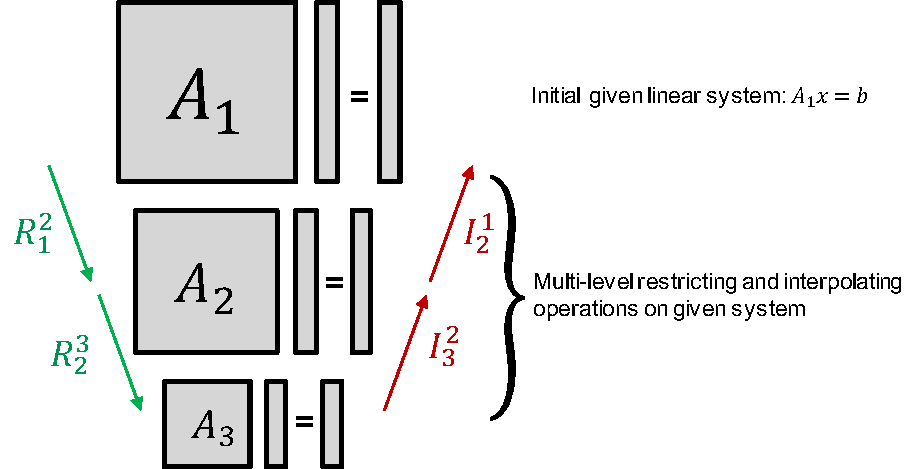
\includegraphics[width=5.6in]{fig/multilevel-amg.pdf}
	\caption{Algebraic multigrid hierarchy.}
	\label{multilevel-amg}
\end{figure}

\subsection{Non-stationary Methods}

In practice, the stationary methods talked in the last section cannot always get the convergence quickly for more general matrices which are not constructed from the Ellipse PDEs. The GMG and AMG which use the relaxation steps of stationary methods' can speed up the convergence for more general matrices, but the construction of restriction, interpolation, and coarse matrices either from geometric PDE problems or the operator matrix $A$ is far more difficult, and these operations matter the convergence. There is no free lunch for AMG which is hard to "control" and get optimal performance. In my dissertation, I will talk more about the \textbf{non-stationary methods} which are easy to implement and have better convergence performance than the stationary methods. The difference of non-stationary methods comparing with stationary methods is that the involved computational information changes at each step of the iteration. The most well-known non-stationary methods are the suite of \textbf{Krylov subspace methods}.

\section{Krylov Subspace methods}

This section presents the Krylov Subspace projection and the basic Arnoldi reduction in the Krylov subspace.

\subsection{Krylov Subspaces}
In linear algebra, the $m$-order Krylov subspace (\cite{saad1981krylov}) generated by a $n\times n$ matrix $A$ and a vector $b$ of dimension $n$ is the linear subspace spanned by the images of $b$ under the first $m$ powers of $A$, that is 
\[K_m(A,b)=span (b, Ab, A^2b,\cdots, A^{m-1}b).\] 

The Krylov subspace provides the ability to extract the approximations from an m-dimensional subspace $K_m$. Since $K_m$ is the subspace of all vectors in $\mathbb{R}^n$, it can be written as $x=p(A)b$, with $p$ a polynomial of degree not exceeding $m-1$.

\subsection{Basic Arnoldi Reduction}

\begin{algorithm}[htbp]{}
	\caption{Arnoldi Reduction}   
	\label{alg:arnoldi-reduction}   
	\begin{algorithmic}[1]
		\Function {AR}{$input$:$A,m,\nu$, $output$: $H_m, \Omega_m$}
		\State $\omega_1=\nu /||\nu||_2$
		\For {\texttt{$j=1, 2, \cdots, m$}}
		\For{$i=1,2,\cdots,j$}
		\State $h_{i,j}=(A\omega_j,\omega_i)$
		\EndFor
		\State $\omega_j=A\omega_j-\sum_{i=1}^jh_{i,j}\omega_i$
		\State $h_{j+1,j}=||\omega_j||_2$
		\If {$h_{j+1,j}=0$} Stop
		\EndIf
		\State $\omega_{j+1}=\omega_j/h_{j+1,j}$
		\EndFor 
		\EndFunction
	\end{algorithmic}  
\end{algorithm}

Arnoldi procedure is well used to build an orthogonal basis of the Krylov subspace $K_m$. One variant of basic Arnoldi reduction algorithm is given in Algorithm \ref{alg:arnoldi-reduction}. In this algorithm, at each step of Arnoldi reduction, the algorithm times the previous Arnoldi vector $\omega_j$ by matrix $A$, and get an orthogonal vector $\omega_j$ against all previous $\omega_i$ by a stand Gram-Schmit procedure. It will stop if the vector computed in line $5$ is zero. Then the vectors $\omega_1, \omega_2. \cdots, \omega_m$ form an orthonormal basis of the Krylov Subspace. 

\begin{figure}[htbp]
	\centering
	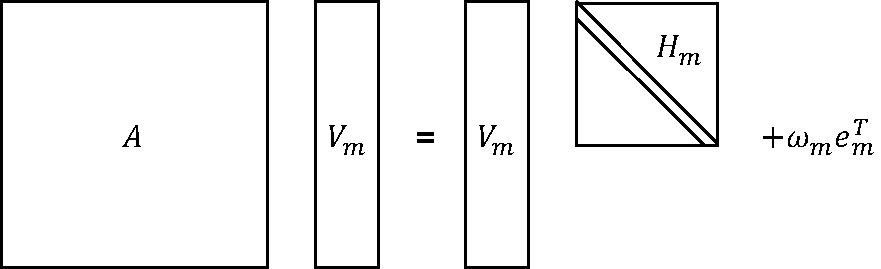
\includegraphics[width=5.8in]{fig/arnoldi_reduction.pdf}
	\caption{ The action of $A$ on $V_m$ gives $V_mH_m$ plus a rank-one matrix.}
	\label{arnoldi}
\end{figure}

Denote by $V_m$, the $n \times m$ matrix with column vectors $\omega_1, \omega_2. \cdots, \omega_m$, by $\overline{H}_m$, the $(m+1) \times m$ Hessemberg matrix whose nonzero entries $h_{i,j}$ are defined by  Algorithm \ref{alg:arnoldi-reduction}, then note $H_m$ as the matrix obtained from  $\overline{H}_m$ by deleting its last row (shown as Fig. \ref{arnoldi}). The following relations are given:
\begin{equation}
AV_m = V_m H_m + \omega_me_m^T = V_{m+1}\bar{H}_m.
\end{equation}

\begin{equation}
V_m^T A V_m = H_m.
\end{equation}

In case that the norm of $\omega_j$ in line $5$ of  Algorithm \ref{alg:arnoldi-reduction} vanishes at a certain step $j$, the next vector $\omega_{j+1}$ cannot be computed and the algorithm steps, $H_m$ turns to be $H_j$ with dimension $j \times j$.


\subsection{Orthogonalization}
There are different orthogonalization schemes to construct the orthogonal basis of Krylov subspace, in this section, we list four variants.

\begin{enumerate}
	\item \textbf{Classic Gram-Schmit Orthogonalization (CGS)}: Algorithm \ref{alg:arnoldi-reduction} gives an example of Arnoldi reduction using the CGS to create a basis vector by vector. The benefit of CGS is the parallelism in computing $h_{i,j}$ and $\omega_j$ in step 5 and 7.
	\item \textbf{Modified Gram-Schmit Orthogonalization (MGS)}: An alternative (See Algorithm \ref{alg:arnoldi-reduction-md}), in which the number of subtractions is reduced, resulting in a less chance of cancellations. Though MGS is more stable than CGS, it is less parallel than CGS. In CGS, the orthogonalization process from line 5 to line 7 can be overlapped, while the same process of MGS has a data dependency. Thus the parallel implementation of Arnoldi reduction still prefers CGS, and a preconditioner or a reorthogonalization process can compensate its deficiency of numerical stability.
	\item \textbf{Householder Orthogonalization}: the  Arnoldi reduction can also be operated by the Householder orthogonalization, which is more numerically robust than the Gram-Schmit orthogonalization.
	\item \textbf{Incomplete Orthogonalization}: The orthogonalization process in Arnoldi is expensive because each vector accumulated in the basis is orthogonalized against all previous ones. Thereby, the orthogonalization process number of iterations $k$ is bounded to the Krylov subspace size, thus higher values of $m$ will imply more computations and memory space in order to create the Krylov orthonormalized vector basis. With the aim to reduce the cost induced by the Arnoldi orthogonalization process, it is possible to truncate it by orthogonalizing each vector against a subset of the basis vectors, i.e. the $q$ precedent basis vectors (Algorithm \ref{alg:arnoldi-incomplete-reduction}). In this case, the resulting upper Hessenberg matrix $H_m$ is not fully orthogonalized and has the propriety to be banded of bandwidth $q$. Incomplete orthogonalization can speed up the construction of Krylov subspace basis, with the loose of numerical accuracy.
\end{enumerate}

\begin{algorithm}[t]{}
	\caption{Arnoldi Reduction with Modified Gram-Schmidt process}   
	\label{alg:arnoldi-reduction-md}   
	\begin{algorithmic}[1]
		\Function {AR-MGS}{$input$:$A,m,\nu$, $output$: $H_m, \Omega_m$}
		\State $\omega_1=\nu /||\nu||_2$
		\For {\texttt{$j=1, 2, \cdots, m$}}
		\For{$i=j,2,\cdots,j$}
		\State $h_{i,j}=(A\omega_j,\omega_i)$
		\State $\omega_j=\omega_j-h_{i,j}v_i$
		\EndFor
		\State $h_{j+1,j}=||\omega_j||_2$
		\If {$h_{j+1,j}=0$} Stop
		\EndIf
		\State $\omega_{j+1}=\omega_j/h_{j+1,j}$
		\EndFor 
		\EndFunction
	\end{algorithmic}  
\end{algorithm}

\begin{algorithm}[t]{}
	\caption{Arnoldi Reduction with Incomplete Orthogonalization process}   
	\label{alg:arnoldi-incomplete-reduction}   
	\begin{algorithmic}[1]
		\Function {AR-Incomplete}{$input$:$A,m,\nu$, $output$: $H_m, \Omega_m$}
		\State $\omega_1=\nu /||\nu||_2$
		\For {\texttt{$j=1, 2, \cdots, m$}}
		\For{$i=max\{1, j - q + 1\},\cdots,j$}
		\State $h_{i,j}=(A\omega_j,\omega_i)$
		\State $\omega_j=\omega_j-h_{i,j}v_i$
		\EndFor
		\State $h_{j+1,j}=||\omega_j||_2$
		\If {$h_{j+1,j}=0$} Stop
		\EndIf
		\State $\omega_{j+1}=\omega_j/h_{j+1,j}$
		\EndFor 
		\EndFunction
	\end{algorithmic}  
\end{algorithm}

\subsection{Krylov Subspace Methods}

The best known Krylov subspace methods are the Arnoldi \cite{voss2004arnoldi}, Lanczos \cite{widlund1978lanczos}, Conjugate gradient \cite{lasdon1967conjugate}, IDR(s) (Induced dimension reduction) \cite{van2015induced}, GMRES (generalized minimum residual), BiCGSTAB (biconjugate gradient stabilized) \cite{sleijpen1993bicgstab}, QMR (quasi minimal residual) \cite{freund1991qmr}, TFQMR (transpose-free QMR) \cite{basermann1996qmr}, and MINRES (minimal residual) \cite{paige1975solution} methods. This dissertation concentrates on GMRES which is used to solve non-Hermitian linear systems.

\section{GMRES for Non-Hermitian Linear Systems}

GMRES is a well-known Krylov iterative method to solve non-Hermitian linear systems $Ax=b$. This section gives an introduction in-depth about the fundamentals of GMRES.

\subsection{Basic GMRES Method}

GMRES (Algorithm \ref{alg:basicgmres}) is a kind of projection method which extracts an approximated solution $x_m$ of given problem in a well-selected $m$-dimensional Krylov subspace \(K_m(A,v)\) from a given initial guess vector $x_0$.  GMRES method was introduced by Youssef Saad and Martin H. Schultz in 1986 \cite{saad1986gmres}.

\begin{algorithm}[htbp]
	\caption{Basic GMRES method}
	\label{alg:basicgmres}
	\begin{algorithmic}[1]
		\Function {BASICGMRES}{$input$: $A, m, x_0,b$, $output$: $x_m$} 
		\State $r_0=b-A x_0, \beta=||r_0||_2$, and $\nu_1=r_0/\beta$
		\State Compute an AR($input$:$A,m,\nu_1$, $output$: $H_m, \Omega_m$)
		\State Compute $y_m$ which minimizes $||\beta e_1-H_m y||_2$ 
		\State $x_m=x_0+\Omega_my_m$
		\EndFunction
	\end{algorithmic}
\end{algorithm}

In fact, any vector $x$ in subspace $x_0+K_m$ can be written as 
\begin{equation}
x = x_0 + V_m y.
\end{equation}

with $y$ an $m$-vector, $V_m$ an orthonormal basis of the Krylov Subspace $K_m$. The norm of residual $R(y)$ of $Ax=b$ is given as:

\begin{equation}
\begin{aligned}
R(y) & = ||b-Ax||_2 =||b-A(x_0+V_m y)||_2 \\&= .||V_{M+1}(\beta e_i - \overline{H}_m y)||_2 = ||\beta e_i - \overline{H}_m y||_2.
\end{aligned}
\end{equation}

The GMRES approximation $x_m$ can be obtained as $x_m = x_0+V_my_m$ where $y_m = argmin_y||\beta e_i - \overline{H}_m y||_2$. The minimizer $y_m$ is inexpensive to compute since it requires the solution of an $(m+1) \times m$ least-squares problem if $m$ is typically small. This gives the basic GMRES method as Algorithm \ref{alg:basicgmres}.

If $m$ is very large, GMRES can be restarted after a number of iterations, to avoid enormous memory and computational requirements with the increase of Krylov subspace projection number. It is called the restarted GMRES. The restarted GMRES won't stop until the condition $||b-Ax_m||<\epsilon_g$ is satisfied. See Algorithm \ref{alg:rgmres} for restarted GMRES algorithm in detail. A well-known difficulty with the restarted GMRES algorithm is that it can stagnate when the matrix is not positive definite. A typical method is to use preconditioning techniques whose goal is to reduce the number of steps required to converge.


\begin{algorithm}[htbp]
	\caption{Restarted GMRES method}
	\label{alg:rgmres}
	\begin{algorithmic}[1]
		\Function {RESTARTEDGMRES}{$input$: $A, m, x_0,b, \epsilon_g$, $output$: $x_m$} 
		\State BASICGMRES($input$: $A, m, x_0,b$, $output$: $x_m$)
		\If {($||b-Ax_m||<\epsilon_g$)} 
		\State Stop
		\Else \State set $x_0 = x_m$ and GOTO 2
		\EndIf
		\EndFunction
	\end{algorithmic}
\end{algorithm}

\subsection{Variants of GMRES}

Several variants of GMRES are proposed, such as:

\begin{enumerate}
	\item \textbf{Restarted GMRES \cite{morgan1995restarted}}: the cost of the iterations grow as $\mathcal{O}(n^2)$, where $n$ is the iteration number. Therefore, the method is sometimes restarted after a number, say $k$, of iterations, with $x_k$ as an initial guess. The resulting method is called Restarted GMRES. This method suffers from stagnation in convergence as the restarted subspace is often close to the earlier subspace.
	
	\item \textbf{Truncated GMRES \cite{de1999truncation}}: a version of GMRES with incomplete orthogonalization, which reduces the computing and memory requirement of the Arnoldi process in GMRES with the cost of the accuracy of orthogonalization.
	
	\item \textbf{Deflated GMRES \cite{erhel1996restarted}}: Restarted GMRES with deflation. As we have just seen, restarting results in a loss of useful information, thus a slowing of convergence after a restart. To overcome this problem, GMRES with deflated restarting (GMRES-DR) was introduced. The deflation in GMRES-DR makes restarted GMRES more robust and makes it converge much faster for tough problems with small eigenvalues.
	
	\item \textbf{Pipelined GMRES \cite{ghysels2014hiding}}: A particular variant of GMRES which hides the global communication latency for parallel implementation.
	
	\item \textbf{FGMRES \cite{fraysse2008algorithm}}: Flexible GMRES presented by Saad is a variant of GMRES with the advantage of being able to switch preconditioners on the fly according to specific heuristics in the GMRES process without any additional computation. This method is interesting because it allows developing robust and easily parallelizable methods. FGMRES is developed based on the right-preconditioner which will be presented later in Section \ref{Left, Right and Split Preconditioning}.
	
\end{enumerate}


\section{Arnoldi for Non-Hermitian Eigenvalue Problems}

The dominant eigenvalues of a non-Hermitian eigenvalue problem can be approximated by the Arnoldi method. In the section, we present the basic algorithm of the Arnoldi method and its variants.

\subsection{Basic Arnoldi Methods}
Arnoldi algorithm \cite{arnoldi1951principle} is widely used to approximate the eigenvalues of large sparse matrices. The kernel of Arnoldi algorithm is the Arnoldi reduction, which gives an orthonormal basis \(\Omega_m = (\omega_1,\omega_2,\cdots,\omega_m)\) of Krylov subspace \(K_m(A,v)\), by the Gram-Schmidt orthogonalization, where \(A\) is  \(n \times n\) matrix, and $\nu$ is a \(n\)-dimensional vector. Since Arnoldi reduction can transfer a matrix \(A\) to be an upper Hessenberg matrix \(H_m\) with relation $V_m^T A V_m = H_m$, the eigenvalues of \(H_m\) are the approximated ones of \(A\), which are called the Ritz values of \(A\). With the Arnoldi reduction, the $r$ desired Ritz values $\Lambda_r=(\lambda_1,\lambda_2,\cdots,\lambda_r)$, and the corresponding Ritz vectors $U_r=(u_1,u_2,\cdots,u_r)$ can be calculated by Basic Arnoldi method.

The numerical accuracy of the computed eigenpairs of basic Arnoldi method depends highly on the size of the Krylov subspace and the orthogonality of $\Omega_m$. Generally, the larger the subspace is, the better the eigenpairs approximation is. The problem is that firstly the orthogonality of the computed $\Omega_m$ tends to degrade with each basis extension. Also, the larger the subspace size is, the larger the $\Omega_m$ matrix gets. Hence available memory may also limit the subspace size, and so the achievable accuracy of the Arnoldi process. To overcome this, Saad \cite{saad2011numerical} proposed to restart the Arnoldi process, which is the ERAM. Inside ERAM, the subspace size is fixed as $m$, and only the starting vector will vary. After one restart of the Arnoldi process, the starting vector will be initialized by using information from the computed Ritz vectors. In this way, the vector will be forced to be in the desired invariant subspace. The Arnoldi process and this iterative scheme will be executed until a satisfactory solution is computed. The Algorithm of ERAM is given by Algorithm \ref{alg:arnoldi}, where $\epsilon_a$ is a tolerance value, $r$ is desired eigenvalues number and the function $g$ defines the stopping criterion of iterations.

\begin{algorithm}[htbp]{}
	\caption{Explicitly Restarted Arnoldi Method}   
	\label{alg:arnoldi}   
	\begin{algorithmic}[1]
		\Function {ERAM}{$input$: $A, r, m, \nu, \epsilon_a$, $output$: $\Lambda_r$} 
		\State Compute an AR($input$:$A,m,v$, $output$: $H_m, \Omega_m$)
		\State Compute $r$ desired eigenvalues $\lambda_i$ ($i  \in [1,r] $) of $H_m$
		\State Set $u_i=\Omega_my_i$, for $i=1,2,\cdots, r$, the Ritz vectors    
		\State Compute $R_r=(\rho_1.\cdots, \rho_r)$ with $\rho_i=||\lambda_i u_i - A u_i||_2$
		\If{$g(\rho_i)<\epsilon_a$ ($i  \in [1,r] $)}
		\State stop
		\Else
		\State set $v=\sum_{i=1}^d Re(\nu_i)$, and GOTO 2
		\EndIf
		\EndFunction
	\end{algorithmic}  
\end{algorithm}

\subsection{Variants of Arnoldi Method}

There are various strategies to restart the basic Arnoldi method and to accelerate the convergence by the deflation of unwanted eigenvalues. This section lists three variants:

\begin{enumerate}
	\item \textbf{Explicitly Restarted Arnoldi Method (ERAM) \cite{morgan1996restarting}}: Arnoldi algorithm restarted explicitly by the combination of Ritz values and vectors.
	
	\item \textbf{Implicitly Restarted Arnoldi Method (IRAM) \cite{sorensen1997implicitly}}: IRAM is a variant of Arnoldi algorithm with deflation of unwanted eigenvalues. It can shift the unwanted eigenvalues of matrix implicitly without the explicit construction of filter polynomial during the process of Arnoldi reduction. The Algorithm \ref{alg:impli-arnoldi} illustrates this method. The shift of unwanted values of matrix $A$ can be transferred to be a shifted QR factorization of Hessemberg matrix $H_m$. IRAM can operate in parallel to solve the large problem without extra memory space.
	
	\item \textbf{Krylov-Schur Method \cite{stewart2002krylov}}: It is another implementation of Arnoldi algorithm with deflation of unwanted eigenvalues. Krylov-Schur method is mathematically equal to IRAM. Its two advantages over IRAM: 1) it is easier to deflate converged Ritz vectors; 2) it avoids the potential forward instability of the QR algorithm. The Algorithm \ref{alg:krylov-schur} gives this method. During the Arnoldi reduction procedure, the Hessemberg matrix $H_m$ is decomposed by the Schur deposition as $H_m=S_mT_mS_m$ with unitary matrix $S_m$ and upper triangular matrix $T_m$. The upper triangular form of $T_m$ eases the analysis of Ritz pairs. The wanted and unwanted Ritz values in $T_m$ can be reordered into two separate parts as $T_{m-k}$ and $T_k$. $T_{m-k}$ can be extended to $m$-dimension without unwanted values through further $k$ steps of Krylov subspace projection. 
	
\end{enumerate}

\begin{algorithm}[t]{}
	\caption{Implicitly Restarted Arnoldi Method}   
	\label{alg:impli-arnoldi}   
	\begin{algorithmic}[1]
		\Function {IRAM}{$input$: $A, r, m, \nu, \epsilon_a$, $output$: $\Lambda_r$} 
		\State Compute an AR($input$:$A,m,v$, $output$: $H_m, \Omega_m$)
		\State Compute the spectrum of $H_m$: $\Lambda (H_m)$. If converge, stop. Otherwise, select set of $p$ shits $\mu_1, \mu_2,\cdots, \mu_p$
		\State $q^T = e_m^T$
		\For{$j=1,2,3,\cdots,p$}
		\State Factor $[Q_J, R_j] = QR(H_m-\mu_jI)$
		\State $H_m = q_j^TH_mQ_j$, $V_m=V_mQ_j$, $q^T=q^TQ_j$
		\EndFor 
		\State $f_k=v_{k+1}H_{m(k+1,k)}+f_mq^T(k)$, $V_k=V_{m(1:n,1:k)}$, $H_k=H_{m(1:k,1:k)}$
		\State Begining with the $k$-step Arnoldi factorization, $AV_k=V_kH_k+f_ke_k^T$, apply $p$ additional steps of the Arnoldi process to obtain a new $m$-step Arnoldi factorization as $AV_m=V_mH_m+f_me_m^T$
		\EndFunction
	\end{algorithmic}  
\end{algorithm}

\begin{algorithm}[htbp]{}
	\caption{Krylov-Schur Method}   
	\label{alg:krylov-schur}   
	\begin{algorithmic}[1]
		\Function {Krylov-Schur}{$input$: $A, x_1, m$, $output$: $\Lambda_k$ with $k \leq p$} 
		\State Build an initial Krylov decompostion of order $m$
		\State Apply orthogonal transformations to get a Krylov-Schur decompostion
		\State Reorder the diagonal blocks of the Krylov-Schur decompostion
		\State Truncate to a Krylov-Schur decompostion of order $p$
		\State Extend to a Krylov decomposition of order $m$
		\State If not satisfied, go to step 3
		\EndFunction
	\end{algorithmic}  
\end{algorithm}


\section{Preconditioners for GMRES}\label{Preconditioners for GMRES}

In practice, one weakness of GMRES discussed in the previous section is the lack of robustness, it is likely to suffer from slow convergence for some problems. Preconditioning is a kind of techniques to accelerate the convergence of Krylov subspace methods by transforming the original linear systems from one to another. In this section, we summarize different kinds of existing preconditioners, including the preconditioning by a selected matrix, by the deflation, and by a selected polynomial.

\subsection{Preconditioning by Selected Matrix}

The first alternative is to use the preconditioning matrix $M$. This $M$ can be defined in many different ways, and it makes it is much easier to solve linear systems $Mx=b$ compared with the original linear systems $Ax=b$. After the selection of $M$, there are three ways to apply this preconditioning matrix $M$ to the original systems: the left, right and split preconditioning.

\subsubsection{Left, Right and Split Preconditioning}\label{Left, Right and Split Preconditioning}

The \textbf{left preconditioning} of matrix on the original linear can be defined as:

\begin{equation}
\label{eqlpgmres}
M^{-1}Ax=    M^{-1}.
\end{equation}

The GMRES is applied to solve the Equation (\ref{eqlpgmres}) instead of the original matrix. The left preconditioned version GMRES is given as Algorithm \ref{alg:lp-gmres}.

\begin{algorithm}[htbp]
	\caption{Left-Preconditioned GMRES}
	\label{alg:lp-gmres}
	\begin{algorithmic}[1]
		\State $r_0=M^{-1}(b-A x_0), \beta=||r_0||_2$, and $\nu_1=r_0/\beta$
		\For{$i=0,\cdots,m-1$}
		\State $z \leftarrow M^{-1}A\nu_i$
		\State $h_{j,i} \leftarrow \langle z,\nu_j\rangle$, $z = z- h_{j,i}\nu_j$ $j=1,\cdots,i$
		\If{$h_{j+1,j} == 0$}
		\State stop
		\Else
		\State {$\nu_{i+1} = z/h_{i+1,i} $, and $h_{i+1,i} = ||z||_2$}
		\EndIf
		\EndFor
		\State Compute $y_m$ which minimizes $||\beta e_1-H_m y||_2$ 
		\State $x_m=x_0+V_my_m$
	\end{algorithmic}
\end{algorithm}

As shown in Algorithm \ref{alg:lp-gmres}, $M$ is applied to each step of GMRES iteration, and the Krylov subspace constructed by the Arnoldi process tends to be:
\begin{equation}
span\{r_0, M^{-1}Ar_0, \cdots, (M^{-1}A)^{m-1}r_0\}.
\end{equation}

The residual vectors in this algorithm can be defined as $r_m=M^{-1}(b-Ax_m)$, instead of the unpreconditioned one $b-Ax_m$.

The \textbf{right preconditioning} of $M$ makes GMRES solve linear systems as follows instead of the original systems:

\begin{equation}
AM^{-1}u=b, \qquad u = Mx.
\end{equation}

The right-preconditioned GMRES is given as Algorithm \ref{alg:rp-gmres}.

\begin{algorithm}[htbp]
	\caption{Right-Preconditioned GMRES}
	\label{alg:rp-gmres}
	\begin{algorithmic}[1]
		\State $r_0=b-A x_0, \beta=||r_0||_2$, and $\nu_1=r_0/\beta$
		\For{$i=0,\cdots,m-1$}
		\State $z \leftarrow AM^{-1}\nu_i$
		\State $h_{j,i} \leftarrow \langle z,\nu_j\rangle$, $z = z- h_{j,i}\nu_j$ $j=1,\cdots,i$
		\If{$h_{j+1,j} == 0$}
		\State stop
		\Else
		\State {$\nu_{i+1} = z/h_{i+1,i} $, and $h_{i+1,i} = ||z||_2$}
		\EndIf
		\EndFor
		\State Compute $y_m$ which minimizes $||\beta e_1-H_m y||_2$ 
		\State $x_m=x_0+M^{-1}V_my_m$
	\end{algorithmic}
\end{algorithm}

As shown in this algorithm, the Krylov subspace spanned by the right preconditioning can be defined as:

\begin{equation}
Span\{r_0, AM^{-1}r_0, \cdots, (AM^{-1})^{m-1}r_0\}.
\end{equation}

The essential difference of right preconditioning comparing with left preconditioning is that the residual vectors in the algorithm can be obtained as $b-Ax_m=b-AM^{-1}u_m$, which is equal the ones of unpreconditioned systems, and independent from the selection of $M$. Thus this preconditioning matrix can vary with different selections for each iteration of GMRES, that is the flexible GMRES, which can be useful for several linear systems.

Another alternative is to use the split preconditioning, which can be seen as a combination of left and right preconditioning. Suppose that a preconditioning matrix $M$ can be factorized as the form:

\begin{equation}
M=LU.
\end{equation}

Then, the split preconditioned linear systems to be solved by GMRES can be defined as:

\begin{equation}
L^{-1}AU^{-1}u=L^{-1}b, \qquad x= U^{-1}u.
\end{equation}

The residual vectors of this type of GMRES is that form $L^{-1}(b-Ax_m)$. In fact, a split preconditioner may be much better if A is nearly symmetric. 

\subsubsection{Jacobi, SOR, and SSOR Preconditioners}

The preconditioners based on stationary methods, such as Jacobi, SOR and SSOR methods is a special collection of left-preconditioners.

The general form for the preconditioning can be given as:

\begin{equation}
x_{k+1} = M^{-1}Nx_k+M^{-1}b,
\end{equation}

where $M$ and $N$ are created by the splitting of $A$ as:

\begin{equation}
A=M-N.
\end{equation}

The above formula can be rewritten as:

\begin{equation}
\label{xgf}
x_{k+1}=Gx_k+f
\end{equation}

with $f=M^{-1}b$ and $G=M^{-1}N=I-M^{-1}A.$

The Expression (\ref{xgf}) is attempting to solve:

\begin{equation}
(I-G)X=f.
\end{equation}


which can be rewritten as:

\begin{equation}
M^{-1}Ax=M^{-1}b.
\end{equation}

For Jacobi Preconditioner, the preconditioning matrix $M$ can be defined as:

\begin{equation}
M_{Jacobi} = D^{-1}.
\end{equation}

For Gauss-Seidel Preconditioner, the preconditioning matrix $M$ can be defined as:

\begin{equation}
M_{Gauss} = (D- E)D^{-1}(D- F).
\end{equation}

For SSOR Preonditioner, the preconditioning matrix $M$ can be defined as:

\begin{equation}
M_{SSOR} =  (D-\omega E)D^{-1}(D-\omega F).
\end{equation}

\subsubsection{Imcomplete LU Preconditioners}

In numerical linear algebra, an incomplete LU factorization (abbreviated as ILU) of a matrix is a sparse approximation of the LU factorization often used as a preconditioner.

For a linear system $Ax=b$, it is often solved by computing the factorization $A=LU$, with $L$ a lower triangular and $U$ upper triangular. One then solves efficiently $Ly=b$ and $Ux=y$ in sequence since $U$, and $L$ are all triangular.  It is well known that usually in the factorization procedure, the matrices L and U have more non zero entries then A. These extra entries are called fill-in entries.

An incomplete factorization \cite{saad1994ilut,sertel2000incomplete, lee2003incomplete,malas2007incomplete} instead seeks triangular matrices $L$ and $U$ such that 
\[A \approx LU.\]

For a typical sparse matrix, the LU factors can be much less sparse than the original matrix - a phenomenon called fill-in. The memory requirements for using a direct solver can then become a bottleneck in solving linear systems. One can combat this problem by using fill-reducing reorderings of the matrix's unknowns, such as the Cuthill-McKee ordering. 

\begin{algorithm}[htbp]
	\caption{Incomplete LU Factorization Algorithm}
	\label{alg:ilu}
	\begin{algorithmic}[1]
		\For{$i=2,\cdots,n$}
			\For {$k = 1, \cdots, i-1$}
				\If {$(i,k) \notin P$}
					\State $a_{i,k} = a_{i,k}/a_{k,k}$
					\For{$j = k+1, \cdots, n$}
						\If{$(i,j) \notin P$}
							\State $a_{i,j} = a_{i,j}-a_{i,k}a_{k,j}$
						\EndIf
					\EndFor
				\EndIf
			\EndFor
		\EndFor
	\end{algorithmic}
\end{algorithm}

Let $S$ be a subset of all positions of the original matrix generally including the main diagonal, and $\forall (i, j)$ such as $a_{i,j} \neq 0$. An incomplete LU factorization of $A$ only allows fill-in positions which are in $S$, which is designated by the elements to drop at each step. $S$ has to be specified in advance in a static way by defining a zero pattern which must exclude the main diagonal. Therefore, for any zero pattern $P$, such that

\begin{equation}
	P \subset \{ (i,j) | i \neq j; 1 \leq i,j\leq n\}
\end{equation}


Solving for $LUx=b$ can be done quickly but does not hield the exact solution to the given problem. So a matrix is \[M_{LU} = LU\]

often used as a preconditioner for another iterative method such as GMRES. For an incomplete factorization with no-fill, named ILU(0), we define the pattern $P$ as the zero pattern of A. However, more accurate factorization can be obtained by allowing some fill-in, denoted by ILU($p$) where $p$ stands for the desired level of fill. This class of preconditioner has some difficulties to converge in a reasonably number of iterations on ill-conditioned systems.

\subsubsection{Preconditioning by Multigrid solvers}

Multigrid methods, including GMG and AMG, are the most complex preconditioners. The MG methods speed up the convergence of stationary iterative methods by smoothing the low-frequency modes of the errors of linear systems with the construction of a series of coarse representations. The main difference between the GMG and AMG is the strategy to construct the restriction, and coarsing matrices. AMG preconditioners need an amount of time for the pre-processing, but they can accelerate convergence much more significantly.

When AMG is applied as a preconditioner (e.g. \cite{plank2007algebraic,leem2004algebraic,yang2002boomeramg,mifune2003new}), the setup phase of restriction matrix $R_h^{2h}$ and the interpolation matrix $I_h^{2h}$ need to be complex as the standalone AMG solvers. The creation of a given number of sub-domains, and each domain representing by only one value at the coarse level is enough. After dividing the nodes of mesh into groups, the projection matrix can be defined as $W$. $W$ is used to build the coarse-system matrix $A_{2h}$ of an original matrix $A$:

\begin{equation}
A_{2h}=W^{T}AW.
\end{equation}

Thus, $W$ is the restriction operation $R_h^{2h}$ , and $W^{T}$ is the interpolation matrix $I_h^{2h}$. After the creation of transfer operation $W$, it can be applied into the Fine-Coarse-Fine loop of MG method to generate an approximate solution of original linear systems. Algorithm \ref{alg:amg-gmres} gives an example of AMG preconditioned GMRES.

\begin{algorithm}[htbp]
	\caption{AMG-Preconditioned GMRES}
	\label{alg:amg-gmres}
	\begin{algorithmic}[1]
		\State $r_0=b-A x_0, \beta=||r_0||_2$, and $\nu_1=r_0/\beta$
		\For{$i=0,\cdots,m-1$}
		
		\State Get $u_p$ by $p$ \textbf{relaxions} on $Au=\nu_i$ starting from $u_0$ using stationary methods.
		\State Find the residual: $r_p=\nu_i - Au_p$.
		\State Project $r_p$ one the coarse level: $r_pc=W^Tr_p$.
		\State Solve the coarse-level residual system: $A_{2h}E_{pc}=r_{pc}$.
		\State Project back $E_{pc}$ the fine level: $E_p = We_{pc}$.
		\State Correct the fine-level approximation: $u_p=u_p+E_p$.
		\State Iterate $p$ times on $Au=\nu_i$ starting from $u_p$, get the final approximation $\hat{u}$.
		\State set $\nu_i = \hat{u}$.
		\State $z \leftarrow A\nu_i$
		\State $h_{j,i} \leftarrow \langle z,\nu_j\rangle$, $z = z- h_{j,i}\nu_j$ $j=1,\cdots,i$
		\If{$h_{j+1,j} == 0$}
		\State stop
		\Else
		\State {$\nu_{i+1} = z/h_{i+1,i} $, and $h_{i+1,i} = ||z||_2$}
		\EndIf
		\EndFor
		\State Compute $y_m$ which minimizes $||\beta e_1-H_m y||_2$ 
		\State $x_m=x_0+M^{-1}V_my_m$
	\end{algorithmic}
\end{algorithm}

\subsection{Preconditioning by Deflation}

It is not always true, but the convergence of Krylov subspace methods for most linear systems, depends to the distribution of eigenvalues. The removing or deflation of the small eigenvalues might greatly improve the convergence performance. In fact, if the dimension of Krylov subspace is large enough, some deflation occurs automatically. But for the restarted GMRES, the limitation of dimension of Krylov subsapce is not enough for these deflation, and convergence cannot be achieved accordingly. Thus deflation schemes should be constructed for each cycle of restart, and this technique is called the deflated preconditioners. Kharchenko et al. \cite{kharchenko1995eigenvalue} built a deflation preconditioner using the approximate eigenvectors. In \cite{erhel1996restarted}, Erhel et al. developed a deflation technique based on an invriant subspace approach; Burrage et al.  \cite{burrage1998deflation} improved this deflation technique by considering the eigenpairs outside the Krylov subsapce of GMRES. Both Chapman et al. \cite{chapman1997deflated} and Gaul et al. \cite{gaul2013framework} presented the deflated and augemented Krylov subspace techniques. Giraud et al. \cite{giraud2010flexible} proposed a novel algorithm that attempts to combine the numerical features of deflated GMRES, and the flexibility of FGMRES. Kutsukake et al. \cite{kutsukake2015deflated} developped a new deflated Flexible GMERS which uses an approximate inverse preconditioner. 

In this section, we given a example of deflated GMRES($m,k$) (denoted as GMRES-DR($m,k$)) developed by Morgan et al. \cite{morgan2002gmres}. GMRES-DR is a deflation preconditioned GMRES uses the thick restarting itea. It has two parameters $m$ and $k$, where $m$ is the restart size of GMRES, and $k$ is the number of eigenvectors used for the deflation during the restart. The first cycle is the same as GMRES($m$), which is able to generate $V_m$ and $H_m$. The $k$ smallest eigenpairs $(\lambda_k, g_k)$ of matrix $H_m+\beta H_m^{-T}e_me_m^T$ can be calculated. Then a matrix $G_k$ can be formulated as:

\begin{equation}
	 G_k=[g_1,g_2,\cdots,g_k]
\end{equation}

and then $G_{k+1}$ can be generated as:

\begin{equation}
	G_{k+1}= ((G_k), c-\bar{H}_my)
\end{equation}

$Q_{k+1}$ can be gotten from $G_{k+1}$, hence $V_{k+1}$ and $H_k$ are generated, where $V_{k+1}$ is a $n \times (k+1)$ matrix and $H_k$ is a $k \times k$ matrix. Therefore, it becomes necessary to extend $V_{k+1}$ and $H_k$ to $V_m$ and $H_m$ by the Arnoldi method that starts at the $k+1$-th iteration. This method is shown in Algorithm \ref{alg:gmres-dr}. GMRES-DR is efficient and numerical stable for deflating the small eigenvalues and accelerate the convergence.

\begin{algorithm}[t]
	\caption{GMRES-DR($A, m,k,x_0$)}
	\label{alg:gmres-dr}
	\begin{algorithmic}[1]
		\State $r_0=b-A x_0, \beta=||r_0||_2$, and $\nu_1=r_0/\beta$
		\For{$i=0,\cdots,m-1$}
		\State $z \leftarrow A\nu_i$
		\State $h_{j,i} \leftarrow \langle z,\nu_j\rangle$, $z = z- h_{j,i}\nu_j$ $j=1,\cdots,i$
		\If{$h_{j+1,j} == 0$}
		\State stop
		\Else
		\State {$\nu_{i+1} = z/h_{i+1,i} $, and $h_{i+1,i} = ||z||_2$}
		\EndIf
		\EndFor
		\State Compute $y_m$ which minimizes $||\beta e_1-H_m y||_2$ 
		\State Compute the $k$ smallest eigenpairs $(\lambda_k, g_k)$ of $H_m+\beta H_m^{-T}e_me_m^T$
		\State Set $G_k=[g_1,g_2,\cdots,g_k]$
		\State Orthonormalize $G_k$ into $Q_{k}$ which is a $n \times k$ matrix
		\State Extend $Q_k$ to length $m+1$ by appending a zero entry to each. Then orthonormalize the vector $c-\bar{H}_m d$ against them to form $q_{k+1}$. Note $c-\bar{H}_m d$ is a vector of length $m+1$, $Q_{k+1}$ can be formulated by combining $Q_k$ and $q_{k+1}$
		\State Set $V_{k+1}^{new} = V_{k+1}Q_{k+1}$ and $\bar{H_{k}}^{new} = Q_{k+1}^H \bar{H_m}$
		\State Reorthogonalize $v_{k+1}$ against the earlier columns of $V_{k+1}^{new}$
		\State Apply the Arnoldi iteration from this point to form the rest of $V_{m+1}$ and $\bar{H}_m$, with $\beta=h_{m+1,m}$
		\State Set $c=V_{m+1}^Tr_0$ and solve $\min||c-\bar{H}_md||_2$ for $d$
		\State Set $x_m=x_0+V_md$, $r_m=b-Ax_m=V_{m+1}(c-\bar{H}_md)$
		\If{$||r_m|| < tol $}
		\State Stop
		\EndIf
		\State  Compute the $k$ smallest eigenpairs $(\lambda_k, g_k)$ of $H_m+\beta H_m^{-T}e_me_m^T$
		\State set $x_0 = x_m$ and Go to Step $1$
	\end{algorithmic}
\end{algorithm}

\subsection{Preconditioning by Polynomials - Introduction in detail on Least Squares Polynomial method}

In the context of iterative methods for solving linear systems, polynomial preconditioners have been studied extensively. In this section, we recall some of the results regarding common polynomial preconditioners, and then give an introduction about the Least Squares Polynomial preconditioner.

\subsubsection{Polynomial Preconditioners for Linear Solvers}

In order to an approximate solution of linear system \[Ax=b,\]one approach is to get the inverse of $A$, denote it as $A^{-1}$, and then the solution gets to be easily obtained as \[x=A^{-1}b\].

Suppose that the characteristic polynomial for $A$:

\begin{equation}
q(A) = \gamma_nA^n+\gamma_{n-1}A^{n-1}+\cdots+\gamma_1A+\gamma_0I = 0.
\end{equation}

The polynomial representation of $A^{-1}$ with $\gamma_0 \neq 0$ can be given as:

\begin{equation}
A^{-1}=\frac{1}{\gamma_0}(-\gamma_nA^{n-1}-\gamma_{n-1}A^{n-1}-\cdots-\gamma_1I)=p(A).
\end{equation}

Therefore, it makes sense to approximate $A^{-1}$ by a polynomial in $A$.  Better selection of this kind of polynomial can approximate more quickly the solution of linear systems.

\subsubsection{Neumann series polynomials}

The simplest $p$ is the polynomial with the Neumann series expansion:

\begin{equation}
I+N^1+N^2+\cdots
\end{equation}

with:

\begin{equation}
N=I-\omega A.
\end{equation}

and $\omega$ is a scaling parameter. The above series can be obtained by the expansion of the inverse of $\omega A$:

\begin{equation}
\begin{aligned}
(\omega A)^{-1} &= [D-(D- \omega D^{-1}A)]^{-1} \\ &= [I-(I- \omega D^{-1}A)]^{-1}D^{-1}. 
\end{aligned}
\end{equation}

where $D$ can be the Identity matrix $I$, the diagonal of $A$, or even a block diagonal of $A$.

Setting:

\begin{equation}
N=I- \omega D^{-1}A,
\end{equation}

and truncating this series, we define a polynomial preconditioner of degree $k$ as:

\begin{equation}
p_{k}(A) = [I+N^1+N^2+\cdots+N^k]D^{-1}.
\end{equation}

Denote the exact solution of $Ax=b$ as $x=A^{-1}b$ and the approximate solution by $p_{k}(A)$ as $x'=p_{k}(A)b$. The error of between $x'$ and $x$ is bounded as:

\begin{equation}
\begin{aligned}
||x-x'|| &= ||A^{-1}b - p_{k}(A)b|| \\ &= ||(I-p_{k}(A)A)A^{-1}b|| \\ &= ||N^{k+1}A^{-1}b|| \leq ||N||^{k+1}||A^{-1}b||.
\end{aligned}
\end{equation}

The performance of precondition by Neumann can be improved with the enlargement of polynomial degree of $p_k$, but matrix operation can be difficult numerically for large $k$.

\subsubsection{Minimum-maximum Polynomials}

In order to accelerate the convergence with the degree $k$ as small as possible, a kind of minimum-maximum polynomials are proposed. Let us define a polynomial preconditioner more abstractly as any polynomial $P_d(A)$ of degree $d$.

The iterates of this polynomial to approximate the solution can be written as 
\begin{equation}
x_d=x_0+P_d(A)r_0.
\end{equation}

Where \(x_0\) is a selected initial approximation to the solution, \(r_0\) the corresponding residual norm, and \(P_d\) a polynomial of degree \(d-1\). We set a polynomial of $d$ degree \(R_d\) such that

\begin{equation}
R_d(\lambda)=1-\lambda P_d(\lambda).
\end{equation}

The residual of \(d^{th}\) steps iteration \(r_d\) can be expressed as equation 

\begin{equation}
r_d=R_d(A)r_0.
\end{equation}

with the constraint \(R_d(0)=1\). We want to find a kind of polynomial which can minimize \(||R_d(A)r_0||_2\), with \(||.||_2\) the Euclidean norm.

If $A$ is a $n \times n$ diagonalizable matrix with its spectrum denoted as \(\sigma(A)=\lambda_1, \cdots, \lambda_n\), and the associated eigenvectors \(u_1, \cdots, u_n\). Expanding the initial residual vector $r_0$ in the basis of these eigenvectors as
\begin{equation}
\label{r0}
r_0=\sum_{i=1}^{n}\rho_i u_i
\end{equation}

moreover, then the residual vector \(r_d\) can be expanded in this basis of these eigenvectors as

\begin{equation}
\label{rn}
r_d=\sum_{i=1}^{n}R_d(\lambda_i)\rho_i u_i
\end{equation}

which allows to get the upper limit of $||r_d||$ as 

\begin{equation}
\label{eq111}
||r_d||_2 \leq ||r_0||_2 \max_{\lambda \in \sigma(A)}|R_d(\lambda)|
\end{equation}

In order to minimize the norm of \(r_d\), it is possible to find a polynomial $P_d$ which can minimize the Equation (\ref{eq111}). And it tends to be a minimum-maximum problem with the constraint \(R_d(0)=1\) and \(\lambda \in  \sigma(A)\)

\begin{equation}
min\ max_{\lambda \in \sigma (A)}|R_d(\lambda)|
\end{equation}

In order to resolve the last problem, a well known method is the Chebyshev iterative method, where \(H\) is taken to be an ellipse with center \(c\) and focal distance \(d\), which contains the convex hull of \(\lambda(A)\). If the origin is outside of this ellipse, the minimal polynomial can be reduced to a scaled and shifed Chebyshev polynomial:

\begin{equation}
R_n(\lambda)=\frac{T_n(\frac{c-\lambda}{d})}{ T_n (\frac{c}{d})}
\end{equation}
The three terms recurrence of Chebyshev polynomial induces an elegant algorithm (shown as Algorithm \ref{alg:hybrid-gmres}) for generating the approximation \(x_n\) that uses only three vectors of storage. But there are servrals constraints with this method, the most important is that the optimal ellipse which encloses the spectrum, often does not accurately represent the spectrum, which may result in slow convergence.

\begin{algorithm}[htbp]
	\caption{Polynomial Preconditioned GMRES}
	\label{alg:hybrid-gmres}
	\begin{algorithmic}[1]
		\State \underline{Start or Restart:}
		\State \hspace{16pt} Compute current residual vector $r=b-Ax$
		\State \underline{Adaptive GMRES step:}
		\State \hspace{16pt} Run $m_1$ steps of GMRES for solving $Ad = r$.
		\State \hspace{16pt} Update $x$ by $x=x+d$.
		\State \hspace{16pt} Get eigenvalue estimates from the eigenvalues of the Hessenberg matrix.
		\State \underline{Compute new polynomial:}
		\State \hspace{16pt} Refine $H$ from previous hull $H$ and new eigenvalue estimates.
		\State \hspace{16pt} Get new best polynomial $p_k$.
		\State \underline{Polynomial Iteration:}
		\State \hspace{16pt} Compute the current residual vector $r= b-Ax$.
		\State \hspace{16pt} Run $m_2$ steps of GMRES applied to $p_k(A)Ad=p_k{A}r$.
		\State \hspace{16pt} Update $x$ by $x=x+d$.
		\State \hspace{16pt} Test for convergence.
		\State \hspace{16pt} If solution converged then Step, else GoTo 1.
	\end{algorithmic}
\end{algorithm}

\subsubsection{Least Squares Polynomial Method}

Based on the normalized Chebyshev polynomial, the Least Squares polynomials methods are introduced. In fact, the spectrum of A is discret, it is possible to introduce one or more polygonal regions without the origin, which has a relatively small number of edges instead of ellipses (\cite{smolarski1982optimum}). The problem tends to find a polynomial \(P_n\) on the boundary of \(H\) which we note as \(\partial H\), that maxmimizes the modulus of \(|1-\lambda P_n(\lambda)|\). And then we get the least square problem with respect to some weight \(w(\lambda)\) on the boundary of \(H\) and the constraint \(R_n(0)=1\).

\begin{figure}[htbp]
	\centering
	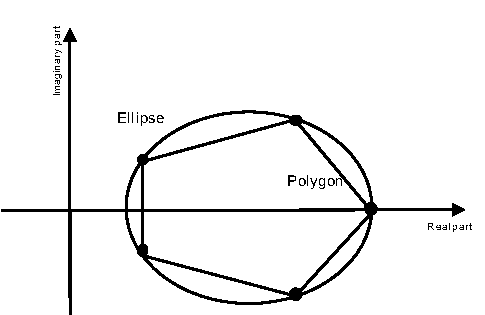
\includegraphics[width=5.4in]{fig/polygon.pdf}
	\caption{The polygon of samllest area containing the convex hull of $\lambda(A)$.}
	\label{polygon}
\end{figure}


\textbf{Weight Function and Gram Matrix}


Suppose that matrix \(A\) is real, we know that its spectrum is symmetric with the real axis, which means we will only need the upper half part \(H^+\) of the convex hull \(H\).

Suppse that \(\partial H^+\) the upper part of boundary \(H\) and \(v=1,\cdots,\mu\) that \(\partial H^+=\cup_{v=1}^\mu E_v\). And then, suppose \(c_v\) and \(d_v\), the center and foscal distance of edge \(E_v\). The inner product of two complex polynomials associated with the weight function \(\omega_v\) on the edge \(E_v\) can be expressed as the expression (11).

\begin{equation}
(p,q)_w=2\Re(\sum_{v=1}^v \int_{E_v}p(\lambda) \overline{q(\lambda)} w_v(\lambda)\mathrm{d}\lambda)
\end{equation}

\begin{equation}
w_v(\lambda)=\frac{2}{\pi}|d_v^2-(\lambda-c_v)^2|^{-\frac{1}{2}}
\end{equation}

The function (12) is the weight function sur one edge \(E_v\) generated by the basis of Chebyshev polynomials (expression 13), which facilite to calculate the inner product.

\begin{equation}
T_i(\frac{\lambda-c_v}{d_v})
\end{equation} 

When we project \(p\) and \(q\) into this basis on the edge \(E_v\), we could get the equations (14) and (15), then the inner product will result into equation (16).

\begin{equation}
p(\lambda)=\sum_{i=0}^n \xi ^v T_i(\frac{\lambda-c_v}{d_v})
\end{equation}

\begin{equation}
q(\lambda)=\sum_{i=0}^n \zeta ^v T_i(\frac{\lambda-c_v}{d_v})
\end{equation}

\begin{equation}
(p,q)_w=2\Re[\sum_{v=1}^\mu 2\xi_0^v \bar{\zeta}_0^v+\sum_{i=1}^\mu 2\xi_1^v \bar{\zeta}_1^v]
\end{equation}

And then, suppose that \(t_j\) the Chebyshev basis on the ellipse \(\xi(c,d,a)\) with \(j \geq 0\), and we can obtain the three terms recurrence with \(i \geq 0\) such as equation (18).

\begin{equation}
t_j(\lambda)=\frac{T_j \frac{\lambda-c}{d}}{T_j \frac{a}{d}}
\end{equation}

\begin{equation}
\beta_{i+1} t_{i+1}(z)=(z-a)t_i(z)-\delta_i t_{i-1}(z)
\end{equation}

With this polynomial basis, we can obtain a so-called modified Gram matrix \(M_n=m_{i,j}\), which is well-conditioned. The entries of \(M_n\) defined by the relation (19) where \(i,j \in 1,\cdots,n+1\), and we can express the inner production formula (16) into the equation (20) with \(\eta=(\eta_1,\cdots,\eta_n)\) and \(\theta=(\theta_1,\cdots,\theta_n)\), which are the coordinates of polynomials \(p\) and \(q\) in basis \(t_i\). 
\begin{equation}
m_{i,j}=(t_{i-1},t_{j-1})_\omega
\end{equation}

\begin{equation}
(p,q)_\omega=(M_n\eta, \theta)
\end{equation}

Expanding the polynomial \(P_n\) into the Chebyshev basis, and then we can get \(R_n\) as equation (22), and in the end we obtain the equation (23) with the three terms recurrence (18). 
\begin{equation}
P_n=\sum_{i=0}^{n-1}\eta_i t_i
\end{equation}

\begin{equation}
\begin{aligned}
R_n(\lambda)&=1-\lambda P_n(\lambda)\\ &=1-\sum_{i=0}^{n-1} \eta_i \lambda t_i(\lambda)
\end{aligned}
\end{equation}

\begin{equation}
\begin{aligned}
R_d(\lambda) =t_0-\sum_{i=0}^{n-1} \eta_i (\beta_{i+1}t_{i+1}+\alpha_i \eta_i + \delta_i \eta_{i+1})t_i.
\end{aligned}
\end{equation}

Then we can can express \(R_n\) into \(e_1-T_n \eta\) with its coordinations in the polynomial \(t_i\), where \(T_n\) is a \((n+1) \times n\) matrix as (24).
\begin{equation}
T_n=
\begin{bmatrix}
\alpha_0       & \delta_1  \\
\beta_1       & \alpha_1 & \delta_2  \\
&  \beta_2 & \alpha_2  & \delta_3\\
& \\
& && &&\delta_{n-1} \\
& && &\beta_{n-1}&\alpha_{n-1} \\
& && &&\beta_{n}
\end{bmatrix}
\end{equation}

With the definition of inner product in the polynomial basis, the function which needs to be minimized can be expressed under the form of equation (25). As \(M_n\) is symmetric, we can get the factorization of \(M_n\) under the form \(M_n=L_n L_n^T\), and in the end we obtain the equation (26) with \(F_n=L_n^TT_k\) a \((n+1) \times n\)upper Hessenberg matrix.
\begin{equation}
\begin{aligned}
||R_n|| &=(R_n,R_n)_\omega \\ &=(M_n(e_1-T_n\eta),e-T_n\eta).
\end{aligned}
\end{equation}

\begin{equation}
\begin{aligned}
||R_n|| &=(R_n,R_n)_\omega \\ &=(L_n^T(e_1-T_n\eta), L_n^T(e_1-T_n\eta)) \\ &=||L_n^T(e_1-T_n\eta)||_2 \\ &=||l_{1,1}-F_n\eta||
\end{aligned}
\end{equation}

The coefficients \(\eta_i\) are the solution of problem \(\min ||l_{1,1}e_1-F_k\eta||_2\) with \(\eta \in IR^n\). This probelm can maybe resolved easily by Givens rotations and QR fatorization. The process to generate the least polynomials by the eigenvalues are given in Algorithm \ref{alg:lsqr-parameters}.

\textbf{Non-Hermitian Linear Systems}

\textcolor{red}{TO DO}

\textbf{Calcul the Iteration Form}

In order to resolve the minimum-maximum problem, a well known method is to use the Chebyshev polynomial, where \(H_k\) is taken to be an ellipse with center \(c\) and focal distance \(d\). This ellipse contains the convex hull of \(\sigma_k(A)\). If the origin is outside of this ellipse, the minimal polynomial can be reduced to a scaled and shifed Chebyshev polynomial:

\begin{equation}
R_d(\lambda)=\frac{T_d(\frac{c-\lambda}{d})}{T_d (\frac{c}{d})}
\end{equation}

The three terms recurrence of Chebyshev polynomial introduces an elegant algorithm for generating the approximation \(x_d\) that uses only three vectors of storage. The choice of ellipses as enclosing regions in Chebyshev acceleration maybe overly restrictive and ineffective if the shape of the convex hull of the unwanted eigenvalues bears little resemblance to an ellipse. There are several reseach to find the acceleration polynomial to minimize its $L_2$-norm on the boundary of the convex hull of the unwanted eigenvalues with respect to some suitable weight function $\omega$. An algorithm based on the modified moments  for computing the least square polynomial was proposed by Youcef Saad \cite{saad1987least}. The problem tends to find a polynomial \(P_d\) on the boundary of \(H_k\) which we note as \(\partial H_k\), that maxmimizes the modulus of \(|1-\lambda P_d(\lambda)|\). And then we get the least square problem with respect to some weight \(w(\lambda)\) on the boundary of \(H_k\) and the constraint \(R_d(0)=1\).

The iteration form of Least Square is \(x_d=x_0+P_d(A)r_0\) with \(P_d\) the least square polynomial of degree \(d-1\) under the Formula (\ref{pd}). The polynomial basis \(t_i\) meet the three terms recurrence relation (\ref{threeterms}). 
\begin{equation}
\label{pd}
P_d=\sum_{i=0}^{d-1}\eta_it_i.
\end{equation}

\begin{equation}
\label{threeterms}
t_{i+1}(\lambda)=\frac{1}{\beta i+1}[\lambda t_i(\lambda)-\alpha_i t_i(\lambda)-\delta_i t_{i-1}]
\end{equation}

For the computation of parameters $H=(\eta_0,\eta_1,\cdots,\eta_{d-1})$, we construct a modified gram matrix $M_d$ with dimension $d \times d$, and matrix $T_d$ with dimension $(d+1) \times d$ by the three terms recurrence of the basis $t_i$. $M_d$ can be factorized to be $M_d=LL^T$ by the Cholesky factorization. The parameters $H$ can be computed by a least squares problem of the formula


\begin{equation}
\label{eq112}
min \|l_{11}e_1-F_d H\|
\end{equation}

We therefore need to compute the vectors \(\omega_i=t_i(A)r_0\), and get the linear combination of formula (\ref{pd}). The recurrence expression of $ \omega_i$ is given as (\ref{omegai}) and the final solution value as (\ref{xd}). The hybrid GMRES preconditioned by least squares polynomial methods is given as Algorithm \ref{alg:hybrid-gmres-ls}.

\begin{equation}
\label{omegai}
\omega_{i+1}=\frac{1}{\beta_{i+1}}(A\omega_i-\alpha_i\omega_i-\delta_i\omega_{i-1})
\end{equation}

\begin{equation}
\begin{aligned}
\label{xd}
x_d &=x_0+P_d(A)r_0 \\ &=x_0+\sum_{i=1}^{d-1}\eta_i\omega_i.
\end{aligned}
\end{equation}

\begin{algorithm}[htbp]
	\caption{Least Square Polynomial Generation}
	\label{alg:lsqr-parameters}
	\begin{algorithmic}[1]
		\Function {LSP}{$input$: $A,b,d,\Lambda_r$, $output$: $A_d, B_d, \Delta_d, H$}
		\State construct the convex hull $C$ by $\Lambda_r$
		\State construct $ellispe(a,c,d)$ by the convex hull $C$
		\State compute parameters $A_d, B_d, \Delta_d$ by $ellispe(a,c,d)$
		\State construct matrix $T$ ${(d+1)} \times d$ matrix by $A_d, B_d, \Delta_d$
		\State construct Gram matrix $M_d$ by Chebyshev polynomials basis
		\State Cholesky factorization $M_d=LL^T$
		\State $F_d=L^TT$
		\State $H_d$ satisfies min $\|l_{11}e_1-F_d H\|$
		\EndFunction
	\end{algorithmic}
\end{algorithm}

\begin{algorithm}[htbp]
	\caption{Hybrid GMRES Preconditioned by Least Squares Polynomial}
	\label{alg:hybrid-gmres-ls}
	\begin{algorithmic}[1]
		\State  Compute current residual vector $r=b-Ax$
		\State Run $m_1$ steps of GMRES for solving $Ad = r$.
		\State  Update $x$ by $x=x+d$.
		\State  Get eigenvalue estimates from the eigenvalues $\Lambda_r$ of the Hessenberg matrix.
		\State  LSP($input$: $A,b,d,\Lambda_r$, $output$: $A_d, B_d, \Delta_d, H$)
		\State  $r_0=f-Ax_0$, $\omega_1 = r_0$ and $x_0=0$
		\For  {$k=1,2,\cdots, s_{use}$}
		\For  {$i=1, 2, \cdots, d-1$}
		\State  $\omega_{i+1}=\frac{1}{\beta_{i+1}}[A\omega_i-\alpha_i\omega_i-\delta_i\omega_{i-1}]$
		\State  $x_{i+1}=x_i+\eta_{i+1}\omega_{i+1}$
		\EndFor
		\EndFor
		\State  set $x_0=x_d$
		\State  Test for convergence.
		\State  If solution converged then Step, else GoTo 1.
	\end{algorithmic}
\end{algorithm}


\section{GMRES Convergence Analysis}

Many things have been proposed over the years to explain GMRES convergence:

\begin{itemize}
	\item Eiegenvalues of $A$;
	\item Pseudo-eigenvalues;
	\item Polynomial numerical hull.
\end{itemize}

This section summarize these discussions.
 
\subsection{Convergence Analysis by Eigenvalues}

\textcolor{red}{TO DO}

G\'erard MEURANT completely describes GMRES convergence for normal matrices. Convergence depends on the eigenvalues of $A$ and on its eigenvectors and $b$ through the weights. 

When $A$ is normal, GMRES convergence depends on the eigenvalues and eigenvectors of $A$. 

\textcolor{red}{TO DO}

GMRES convergence is governed by the distribution of the eigenvalues of $V^TW$ on the unit circle (and also the weights $\omega_i$).  When $A$ is non-normal, GMRES convergence depends on the eigenvalues and eigenvectors of $Q=V^TW$.

\begin{theorem}
	Denote $x_m$ be the approximate solution obtained from the $m$-th step of GMRES, and the related residual is $r_m=b-Ax_m$. Then, $x_m$ is of the form:
	
	\begin{equation}
		x_m = x_0 + q_m(A)r_0
	\end{equation}
	
	and 
	\begin{equation}
		||r_m||_2=||(I-Aq_m(A))r_0||_2=\min_{q \in \mathbb{P}_{m-1}}||(I-Aq(A))r_0||_2
	\end{equation}
\end{theorem}

\begin{theorem}
	If $A$ is a $n \times n$ diagonalizable matrix and let $A=P\Lambda P^{-1}$ with $\Lambda=diag{\lambda_1, \lambda_2, \cdots, \lambda_n}$ is the diagonal matrix of eigenvalues. Then the residual norm achieved by the $m$-th step of GMRES satisfies the inequality
	
	\begin{equation}
		||r_m||_2 \leq c_2(P)\epsilon^{(m)}||r_0||_2.
	\end{equation}
\end{theorem}

where $\epsilon^{(m)}=\min_{p \in \mathbb{P}_m, p(0)=1} \max_{\lambda \in \sigma(A)i=1,\cdots,n}|p(\lambda_i)|$, and $c_2(P)=||P||_2||P^{-1}||_2$.

The exact proof can be found in \cite{saad2003iterative}.

\subsection{Convergence Analysis by Pseudo-eigenvalues}

\subsection{Convergence Analysis by Polynomial Numerical Hull}


\begin{corollary}
	If $A$ is a $n \times n$ diagonalizable matrix and let $A=P\Lambda P^{-1}$ with $\Lambda=diag{\lambda_1, \lambda_2, \cdots, \lambda_n}$ is the diagonal matrix of eigenvalues. Assume that all the eigenvalues of $A$ are located in the ellipse $E(c,d,a)$ which excludes the origin. The residual norm achieved at the $m$-th step of GMRES satisfies the inequality.
	
	\begin{equation}
	||r_m||_2 \leq c_2(P)\frac{C_m(\frac{a}{d})}{|C_m\frac{c}{d}|}||r_0||_2.
	\end{equation}
\end{corollary}

\section{Parallel Krylov methods on Large-scale Supercomputers}

Krylov subspace methods are generally implemented in parallel on the supercomputers to solve very large linear systems and eigenvalue problems. This section discusses the scheme to implement Krylov methods in parallel.

\subsection{Core Operations in Krylov Methods}

It is necessary to identify the main operations in Krylov methods before the parallel implementation. Consider Algorithm \ref{alg:arnoldi-reduction}, \ref{alg:basicgmres} and \ref{alg:arnoldi}. We distinguish four types of operations, which are:

\begin{itemize}
	\item Matrix-vector products in step $5$ of Algorithm \ref{alg:arnoldi-reduction};
	\item AXPY operation in step $7$ of Algorithm \ref{alg:arnoldi-reduction};
	\item Dot products in step $8$ of Algorithm \ref{alg:arnoldi-reduction};
	\item Orthogonalization of vector for the loop from step $4$ to $6$ in of Algorithm \ref{alg:arnoldi-reduction}.
\end{itemize}

This section gives the parallel implementation of these four operations in details.

\subsubsection{AXPY Operation}

AXPY is in the form:

\begin{equation}
y = \alpha x + y.
\end{equation}

With $x$ and $y$ two vectors, and $\alpha$ is a scalar. This operation is used to \textit{update vectors} inside Krylov subspace methods. On distributed memory platforms, it is necessary to assume that the vectors $x$ and $y$ should be distributed in the same manner across all the processor. The distributed AXPY is simple without requiring communication. It can be regarded as several AXPY of local vectors in serial on each processor.

\subsubsection{Dot product and Global Reduction Operation}

The dot product is the operation that use all the components of given vectors to compute a single floating-point scalar. In the Arnoldi reduction process, this scalar is always needed by all processors. Equation (\ref{dotproduct}) gives the formula of dot product operation.

\begin{equation}
\label{dotproduct}
v\cdot w = \langle v_1, v_2, \cdots, v_n \rangle \cdot\langle w_1, w_2, \cdots, w_n\rangle = v_1w_1+v_2w_2+\cdots+v_nw_n.
\end{equation}
The distributed version of the dot-product is needed to compute the inner product of two vectors $v$ and $w$ and then distribute the result across all the processors.  This types of operations are termed the \textit{All Reduction Operations}, which can be seen as the combination \textit{Reduction Operations} and \textit{Broadcast Operations}. In Krylov subspace methods, the dot-product operation is typically needed to perform the vector update on each processor. If the number of processors is large, this kind of operations can introduce enormous communication costs. The computation of the Euclidean norm of distributed vectors is also a global reduction operation which is similar to the dot-product.

\subsubsection{Orthogonalization of Vector}

In the Arnoldi reduction (as shown by Algorithm \ref{alg:arnoldi-reduction}) for non-Hermitian matrices, the vector $Av_i$ should be orthogonalized against all the previous vectors. In practice, the classic Gram-Schmidt process is preferred than the Modified Gram-Schmidt, even the presence of round-offs and cancellations within CGS diminish its numerical stability. In CGS, the orthogonalization process is overlapped, while the same process of MGS has a data dependency, which is not possible to get good parallel performance. A preconditioner or a reorthogonalization process can compensate the deficiency of numerical stability.

\begin{figure}[h]
	\centering
	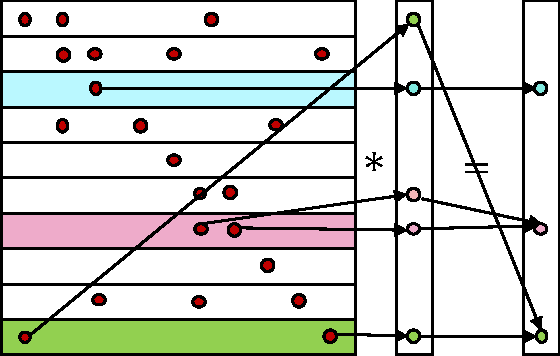
\includegraphics[width=4.8in]{fig/spmv.pdf}
	\caption{Communication Scheme of SpMV.}
	\label{fig:spmv}
\end{figure}

\subsubsection{Matrix-vector products}

In practice, the parallel version of Arnoldi orthogonalization is memory/communication bounded. The most critical operation with the high communication intensity is the substantial number of matrix-vector multiplications $Av_i$. Krylov subspaces are often used to solve linear systems and eigenvalue problems associated with the sparse matrix. Its parallel implementation depends heavily on the data structure to store the matrix. Different distributed sparse matrix format introduces different matrix-vector implementation scheme and finally results in the different parallel performances.

The standard used sparse matrix storage format includes: COO (Coordinate lists) which stores respectively the row index, column index and values into three arrays; CSR (Compressed Sparse Row) which stores respectively the row offset, the column index and data values into three arrays; ELLPACK which stores the column index and values into two two-dimensional arrays according their row index; and DIA (Diagonal format) which store the diagonal offsets into one-dimensional array, and the values sorted by diagonal into a two-dimensional array.

For the parallel implementation of SpMV on modern parallel systems, the matrix with selected storage format should be distributed across different processors with considering the load balance and reduction of communications. Fig. \ref{fig:spmv} gives the communication scheme of SpMV on distributed memory memory systems.

\begin{figure}[h]
	\centering
	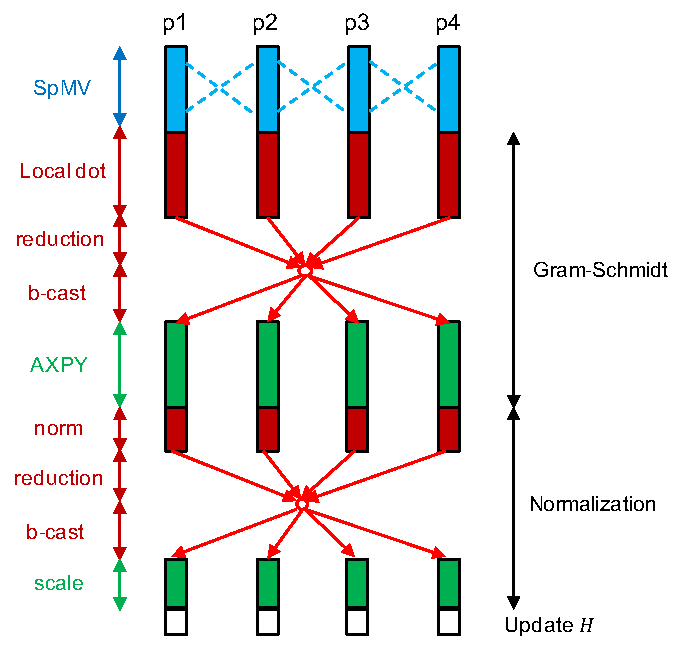
\includegraphics[width=5.4in]{fig/parallel_gmres.pdf}
	\caption{Classic Parallel implementation of Arnoldi reduction.}
	\label{parallel_gmres}
\end{figure}

\subsubsection{Parallel GMRES on Distributed Memory Systems}

Fig. \ref{parallel_gmres} describes the parallel implementation of the Arnoldi reduction process inside GMRES.  For each loop inside, it can be divided into two parts: the Gram-Schmidt and the normalization processes. The SpMV in Gram-Schmidt process is implemented in parallel with the communication among the processors, and the distributed version of dot-product operation is the combination of \textit{Reduction} and \textit{Broadcast} Operations, which introduce a synchronization point, and the AXPY is implemented in parallel without communications. In the normalization process, the computation of the norm of the distributed vectors also introduce the synchronization points. In the Arnoldi reduction, this loop is executed in sequence for $m$ times to generate an orthonormal basis in the $m$-dimensional Krylov subspace.

\subsection{Existing Softwares}

Recent years, there are several efforts to provide the parallel Krylov methods on different computing architectures. This section gives a glance at two famous ones of them.

\subsubsection{PETSc/SLEPc} 

The \textbf{Portable, Extensible Toolkit for Scientific Computation (PETSc)} \cite{balay2001petsc}, is a suite of data structures and routines developed by Argonne National Laboratory for the scalable (parallel) solution of scientific applications modeled by partial differential equations. It employs the Message Passing Interface (MPI) standard for all message-passing communication. PETSc provides many of the mechanisms needed within parallel application code, such as simple parallel matrix and vector assembly routines that allow the overlap of communication and computation. PETSc provides the parallel implementation of Krylov methods and several preconditioners.

The \textbf{Scalable Library for Eigenvalue Problem Computations (SLEPc)} \cite{hernandez2005slepc} is a software library for the parallel computation of eigenvalues and eigenvectors of large, sparse matrices. It can be seen as a module of PETSc that provides solvers for different types of eigenproblems, including linear (standard and generalized) and nonlinear (quadratic, polynomial and general), as well as the SVD. Recent versions also include support for matrix functions. It uses also the MPI standard for parallelization. Both real and complex arithmetic are supported, with single, double and quadruple precision. When using SLEPc, the application programmer can use any of the PETSc's data structures and solvers. Other PETSc features are incorporated into SLEPc as well. The module \textit{EPS} in SLEPc provides Krylov subspace methods such as Krylov-Schur, Arnoldi and Lanczos to solve sparse eigenvalue problems.

\subsubsection{Trilinos} 

\textbf{Trilinos} \cite{heroux2005overview} is a collection of open-source software libraries, intended to be used as building blocks for the development of scientific applications. The word "Trilinos" is Greek and conveys the idea of "a string of pearls," suggesting a number of software packages linked together by a common infrastructure. Trilinos was developed at Sandia National Laboratories from a core group of existing algorithms and utilizes the functionality of software interfaces such as the BLAS, LAPACK, and MPI (the message-passing interface for distributed-memory parallel programming). Fortunately, Trilinos supports many different packages which are defined to implement the iterative linear and eigen-solvers methods. There are some packages which are widely used as follows:

\begin{itemize}
	\item \textbf{Kokkos \cite{edwards2014kokkos}}: Kokkos Core implements a programming model in C++ for writing performance portable applications targeting all major HPC platforms. For that purpose, it provides abstractions for both parallel executions of code and data management. Kokkos is designed to target complex node architectures with N-level memory hierarchies and multiple types of execution resources. It currently can use OpenMP, Pthreads, and CUDA as backend programming models.
	\item \textbf{Epetra \cite{heroux2005epetra}}: Epetra provides the fundamental construction routines and services function that are required for serial and parallel linear algebra libraries. Epetra provides the underlying foundation for all Trilinos solvers.
	
	\item \textbf{Tpetra \cite{baker2012tpetra}}: Tpetra is the next version of Epetra with better support for shared-memory parallelism. It implements linear algebra objects including sparse graphs, sparse matrices, and dense vectors.  Many Trilinos packages and applications produce, modify, or consume Tpetra’s linear algebra objects, or depend on Tpetra’s parallel data redistribution facilities. Tpetra is “hybrid parallel,” meaning that it uses at least two levels of parallelism: MPI  for distributed-memory parallelism and Any of various shared-memory parallel programming models within an MPI process, Tpetra uses the Kokkos package’s shared-memory parallel programming model for data structures and computational kernels.  Kokkos makes it easy to port Tpetra to new computer architectures and to extend its use of parallel computational kernels and thread-scalable data structures.  Kokkos supports several different parallel programming models, including OpenMP, POSIX Threads and Nvidia’s CUDA programming model for graphics processing units (GPUs). Tpetra has the following unique features:
	
	\begin{itemize}
		\item Native support for representing and solving very large graphs, matrices, and vectors.  “Very large” means over two billion unknowns or other entities;
		\item Matrices and vectors may contain many different kinds of data, such as floating-point types of different precision and complex-valued types;
		\item Support for many different shared-memory parallel programming models based on Kokkos.
	\end{itemize}
	
	\item \textbf{AztecOO \cite{heroux2004aztecoo}}: Preconditioners and Krylov subspace methods (conjugate gradient, GMRES, etc.), compatible with Epetra only.
	\item \textbf{Belos \cite{bavier2012amesos2}}: Classical and block Krylov subspace methods (implementations of iterated classical Gram-Schmidt (ICGS), classical Gram-Schmidt with a DGKS correction step, implementations of conjugate gradient (CG), block CG, block GMRES, pseudo-block GMRES, block flexible GMRES, and GCRO-DR iterations). Belos is compatible with Epetra and Tpetra.
	\item \textbf{Anasazi \cite{baker2009anasazi}}: Parallel eigensolvers, Anasazi is compatible with Epetra and Tpetra. It is a package within the Trilinos Project that uses ANSI C++ and modern software paradigms to implement algorithms for the numerical solution of large-scale eigenvalue problems.
	\item \textbf{Komplex \cite{day2001solving}}: Complex-valued system solver, KOMPLEX is an add-on module to AztecOO that allows users to solve complex-valued linear systems. KOMPLEX solves a complex-valued linear system Ax=b by solving an equivalent real-valued system of twice the dimension.
\end{itemize}

\section{Toward Extreme Computing, Some Correlated Goals}\label{Toward Extreme Computing, Some Correlated Goals}
%Global vs Local Communication, fault tolerance, multiple level parallellism, etc. 

This section gives the challenges of numerical methods facing the development of HPC platforms. In Section \ref{Exascale Challenges of Supercomputers}, we discussed the tendance of future exascale supercomputing architectures and the related challenges of parallel programming to develop the applications to profit efficiently from these supercomputers. The main objective for the parallel implementation of numerical methods is to minimize the global computing time. The global computing time of an algorithm can be reduced by either accelerating the convergence or improve its parallel scaling performance using much more computing units. In section, we list in details the correlated goals of iterative methods toward the extreme computing below:

\begin{enumerate}
	
	\item \textbf{Accelerate the convergence}: When solving linear systems by Krylov subspace, the convergence cannot be guranteed for the ill-conditioned matrix or the restart strategy all used. Thus, one important issue for the iterative methods is to propose different kinds of preconditioners which have better speedup on the convergence, and also enough numerical stability. Moverover, facing the comping exascale computing, the proposed preconditioners should either with better parallel performance across large number of cores, or be able to promote the asynchronisity, and benefit from the more complex architectures of mordern supercomputers. 
	
	\item \textbf{Minimize the number of communications}: When solving very large problems on parallel architectures, the most significant concern becomes the cost per iteration of the method -- typically because of communication and synchronization overheads. In general, the complexity of algorithms (number of operations performed) is used to express their performance rather than the quantity of data movement and communications. In fact, on the exascale computers, the global communications accross millinos of cores are very expensive and the computing operations inside each core will be nearly free. To address the critical issue of communication costs, researchers need to investigate algorithms that minimize communication. Considering inside the Krylov iterative methods such as such as GMRES, CG, and Lanczos, the operations of loop inside Arnoldi reduction much more global communications. 
	
	When matrix $A$ in Krylov subspace methods is very sparse, the sparse matrix-vector multiplication (SpMV) invokes even more communications. Hence, strategies for reducing communication overheads in Arnoldi orthogonalization have been proposed to address this bottleneck. In order to reduce the global communication of SpMV for sparse matrices, the first approach is to select the best sparse matrix storage format, which can produces less communications (e.g. \cite{montagne2004optimal, liu2015csr5,stathis2003hierarchical,merrill2016merge,bell2008efficient, bell2009implementing,kreutzer2014unified,ashari2014efficient}). Another approach is to use the Hypergraph Partitioning Models to optimize the SpMV scheme on parallel computers, e.g. in 1999, Catalyurek et al. proposed two computational hypergraph models which avoid this crucial deficiency of the graph model for SpMV \cite{catalyurek1999hypergraph}; Vastenhouw et al. tried to reduce the communication volume of SpMV through a recursive bipartitioning of the sparse matrix \cite{vastenhouw2005two}; Chen et al. proposed a communication optimization scheme based on the hypergraph for basis computation of krylov subspace methods on multi-GPUs \cite{chen2014communication}; a Locality-aware parallel sparse matrix-vector and matrix-transpose-vector multiplication on many-core processors is introduced by Karsavuran et al. \cite{karsavuran2016locality}; and spatiotemporal graph and hypergraph partitioning models for SpMV on manycore architectures is presented by Abubaker et al. with better scaling performance through enhancing data locality in the operations \cite{abubaker2018spatiotemporal}, etc.
	
	\item \textbf{Promote the asynchronisity and reduce the synchronization}: One alogrithm often must do the synchronize operations during the computation. The global data synchronization across amount of cores in the distributed memory systems is expensive especially for a hybrid platform with accelerators. Inside Krylov subspace methods, dot product is a good example which needs the global synchronization after its \textit{global reduction}. For the extreme-scale platforms, synchronizations become bottlenecks. Hence, the algorithm should be designed with as few synchronization points as possible.
	
	Attempts have been made to restructure existing algorithms for the exascale computing so that the number of synchronizations is reduced. Communication-avoiding and pipelined variants of Krylov solvers are critical for the scalability of linear system solvers on future exascale architectures. Firstly, the impact of global communication latency at extreme scales on Krylov methods are analyzed by Ashby et al. \cite{ashby2012impact}. The strategy of hiding global synchronization latency in GMRES and the preconditioned CG was presented by Ghysels \cite{ghysels2013hiding,ghysels2014hiding}; Fujino et al. evaluated performance of parallel computing of revised BiCGSafe and BiCGStar-plus method, and made clear that the revised single synchronized BiCGSafe method outperforms other methods from the view points of elapsed time and speedup on parallel computer with distributed memory \cite{fujino2015estimation}; Rupp et al. implemented pipelined iterative solvers with kernel fusion for GPUs \cite{rupp2016pipelined}; Sanan et al. presented variants of CG, CR, GMRES which both piplined and flexible (\cite{sanan2016pipelined}); Yamazaki et al. proposed to improving the performance of GMRES by reducing communication and pipelining global collectives \cite{yamazaki2017improving}; Swirydowicz et al. presented low synchronization variants of iterated classical (CGS) and modified Gram-Schmidt (MGS) algorithms that require one and two global reduction communication steps; the reduction operations are overlapped with computations and pipelined to optimize performance \cite{swirydowicz2018low}, etc. Moreover, on important considerationin for the restructuring an algorithm to reduce synchronization and communication is their numerical stability.
	
	\item \textbf{Memory and cache optimization for the heterogeneity and scale}: Extracting the desired performance from environments that offer massive parallelism, especially where additional constraints (e.g., limits on memory bandwidth and energy) are in play, requires more sophisticated scheduling and memory management techniques than have heretofore been applied to linear algebra libraries. Confronting the limits of domain-decomposition in the face of massive, explicit parallelism introduces another form of heterogeneity. Feed-forward pipeline parallelism can be used to extract additional parallelism without forcing additional domain-decomposition, but it exposes the user to dataflow hazards. Ideas relating to a data-flow-like model, where parallelism is expressed explicitly in DAGs, allows for dynamic scheduling of tasks, support of massive parallelism, and application of common optimization techniques to increase throughput. Approaches for isolating side-effects include explicit approaches that annotate the input arguments to explicitly identify their scope of reference and implicit methods, such as using language semantics or strongly typed elements to render code easier to analyze for side-effects by compiler technology. New primitives for memory management techniques are needed that enable diverse memory management systems to be managed efficiently and in coordination with the execution schedule.
	
	\item \textbf{Mixed arithmetic}: One important for the development of numerical methods for the exascale computing is to recognize and exploit the presence of mixed-precision mathematics. Low-precision floating-point arithmetic is a powerful tool for accelerating scientific computing applications, especially those in artificial intelligence. In fact, on the modern computing architectures, the 32-bits operation can achieve at least two times speedup over the performance of 64-bits operations. Additionaly, through the combination of 32-bits and 64-bits floating-point arithmetic, where the performance of many linear algebra algorithms can be significantly enhanced by the 32-bits precision operations while maintaining the 64-bit accuracy of the resulting solution. The mixed archmetic can be applied to the different computing architectures including the conventional CPUs and the accelerators such as GPUs. The creation of mixed-precision algorithms allows more effectively utilizing of the heterogeneous hardwares. Little modification of exsiting codes can provide signficant speedup by taking into account existing hardware properties. 
	
	In 2014, Kouya et al. \cite{kouya2014highly}, evaluate the performance of Krylov subspace methods by using highly efficient multiple precision SpMV. They show that SpMV implemented in these functions can be more efficient. \cite{yamazaki2015mixed}, Yamazaki present a mixed-precision Cholesky factorization, which has $1.4\times$ speedup over the standard approach on GPU. Additionaly, their studies of  using the mixed-precision Cholesky factorization within communication-avoiding variants of Krylov subspace projectionmethods demonstrate that by using the higher precision for this small but critical segment of the Krylov methods, we can improve not only the overall numerical stability of the solvers but also, in some cases, their performance. In 2018, Haidar et al. \cite{haidar2018harnessing} investigate how HPC applications can be accelerated by the mixed arithmetic technique. In details, they developed the architecture-specific algorithms and highly tuned implementations of a solver based on mixed-precision (FP16-FP64) iterative refinement for the general linear system, $Ax=b$, where $A$ is a large dense matrix, and a double precision (FP64) solution is needed for accuracy. Their paper show how using half-precision Tensor Cores (FP16-TC) for the arithmetic can provide up to $4\times$ speedup. Maynard et al.  \cite{maynard2018precision} present a mixed-precision implementation of Krylov solver for the numerical weather prediction and climate modelling, the beneficial effect on run-time and the impact on solver convergence. The complex interplay of errors arising from accumulated round-off in floating-point arithmetic and other numerical effects is discussed. They employ now the mixed-precision solver in the operational forecast to satisfy run-time constraints without compromising the accuracy of the solution.
	
	\item \textbf{Minimize energy consumption}: The generated heat also affects the performance of clusters such as the arising failure rate of hardware, and the energy consumption also becomes a tremendous financial burden for supercomputer centers, because it takes up a large portion in the total cost of ownership (TCO), that is the \textit{Power wall}, another roadrock to approach the exascale computing. The HPC community starts to address this problem in recent years, and it is necessary to build power and energy awareness, control, and efficiency of numerical methods and libraries. 
	
	In 2013, an analysis of energy-optimized lattice-Boltzmann CFD simulations from the chip to the highly parallel level is introduced by Wittmann et al. \cite{wittmann2013analysis}. Padoin et al. \cite{padoin2013evaluating} evaluated the application performance and energy consumption on hybrid CPU+ GPU architecture. In 2015, Anzt et al. \cite{anzt2015energy} unveil some energy efficiency and performance frontiers for sparse computations on GPU-based supercomputers. Aliaga et al. \cite{aliaga2015unveiling} unveil the performance-energy trade-off in iterative linear system solvers for multithreaded processors. In order to gain insights about the benefits of hands-on optimizations, they analyze the runtime and energy efficiency results for both out-of-the-box usage relying exclusively on compiler optimizations, and implementations manually optimized for target architectures,that range from CPUs and DSPs to manycore GPUs.
	
	\item \textbf{Multi-level Parallelism}: 
	
	\item \textbf{Adaptive response to load imbalance}: For the exascale computing with millinons of cores and accelerators, even naturally load-balanced algorithms on homogeneous hardware will present many of the same load-balancing problems. Dynamic scheduling based on directed acyclic graphs (DAGs) has been identified as a path forward, but this approach will require new approaches to optimize for resource utilization without compromising spatial locality. The current implementation DAGs based runtime including StarPU \cite{augonnet2011starpu}, OmpSs \cite{duran2011ompss}, etc.
	
	\item \textbf{Autotuning}: Numerical algorithms and libraries need the ability to adapt to the possibly heterogeneous environment in which they operate. Such adaptation must deal with the complexity of discovering and applying the best algorithm for diverse and rapidly evolving ar- chitectures. An automated process would be best, both for productivity and for correctness, where productivity refers both to the development time of the implementation and to the user’s time to solution. The objective is to provide a consistent library interface that, independent of scale and processor heterogeneity, can achieve good performance and efficiency by binding to different under- lying code, depending on the configuration. The diversity and rapid evolution of today’s platforms mean that autotuning of libraries such as the BLAS will be indispensable to achieving good perfor- mance, energy efficiency, and load balancing across the range of systems. In addition, autotuning has to be extended to frameworks that go beyond libraries, such as optimizing data layout (e.g., blocking strategies for sparse matrix/SpMV kernels), stencil autotuners (since stencils kernels are diverse and not amenable to library calls), and even tuning of the optimization strategy for multigrid solvers (optimizing the transition between the multigrid coarsening cycle and bottom-solver to minimize runtime). Adding heuristic search techniques and combining these with traditional compiler techniques will enhance the ability to address generic problems extending beyond linear algebra.
	
	Aquilanti et al. \cite{aquilanti2011parallel} present a general parallel auto-tuned linear solver approach based on the tuning of the Arnoldi incomplete orthogonalization process within GMRES by monitoring the convergence in order to reduce the time of computation needed for a solver to attain solution. Katagiri et al. \cite{katagiri2012smart} presented a smart tuning strategy for restart frequency of GMRES with hierarchical cache sizes.
	
	\item \textbf{Fault tolerance, resilience}: Computing an incorrect answer quickly is of no use to a scientist. Yet computing with exascale hardware poses several challenges in assessing and assuring the correctness of numerical simulation results. Resilience to faults has been identified as a critical need for future HPC systems [57]; the thousandfold increase in computational capabilities expected over the next decade, along with incorporation of techniques for reducing energy consumption, is predicted to increase the error rate of the largest systems. DOE has several critical mission deliverables, including annual stockpile certification and safety assurance for the NNSA and future energy generation technologies for the Office of Science. Computer simulations are key to meeting these deliverables and must be resilient enough to complete in time and correctly, in order to meet the respective critical mission need. In many cases, these simulations can take days, weeks, or even months to complete, which increases the computation’s exposure to faults. Both hard and soft faults are expected to occur with much greater frequency than on previous hardware. Uncorrected soft faults have the potential to corrupt computed solutions. Hard faults will need to be handled on the fly; halting and restarting an entire application because of the loss of a node, for instance, will be prohibitively expensive at the exascale. Dynamically recovering from either type of fault will introduce nondeterministic variability in resource usage, as will dynamic scheduling of tasks. Because of the nonassociativity of floating-point arithmetic, such nondetermin- ism will make bitwise reproducibility difficult at best and will complicate code correctness testing procedures, including code verification, where reproducible execution behavior is assumed. Preventing all faults during exascale simulation will be impossible, and nondeterministic execu- tion is likewise unavoidable without potentially severe performance penalties. Fault management will require developments in hardware, programming environments, runtime systems, and pro- gramming models; but mathematics will play an important role as well. The issue of correctness is ultimately a mathematical one and will require mathematics-informed solutions. Research will be required in order to devise efficient application-level fault-tolerance mechanisms and new procedures to verify code correctness at scale.

\end{enumerate}

The work of this dessertition try to propose a potential smart multi-level parallel programming with auto-tuning scheme for solving linear systems which address on the goals of acceleration of convergence, minimizing the number of communications, promoting the asynchronisity, reducing the synchronize points and fault tolerance.

\clearemptydoublepage